\todo[inline]{For each thing you explain also say why you explain it, what role will it play later in this thesis}

\section{In computer science and in software engineering}
\paragraph{Agile Methodology}
The Agile methodology is a set of techniques and principles for conducting a development project. The main principle is to iterate over short periods (called sprints) divided in subphases in order to build the final product in an incremental way.
A sprint lasts between one and two weeks and is divided as follows: 
\begin{itemize}
    \item At the start of each iteration, we plan with the client what we are going to do this iteration.
    \item Next step is to think about how to build a good design to achieve the objective
    \item Then, we develop the features
    \item After, we test these features. If we switch these last two steps, we apply what is called Test-Driven Development. With this methodology, a team write tests before developing the corresponding features, ensuring that the tests will cover all the cases
    \item At the end of each sprint, we meet the client again to validate the changes and new features, collect his feedback about the project's progress and to define together the future work.
\end{itemize}
A visual representation of this iterative approach is shown on figure \ref{fig:agile-methodology}


\begin{figure}
    \centering
    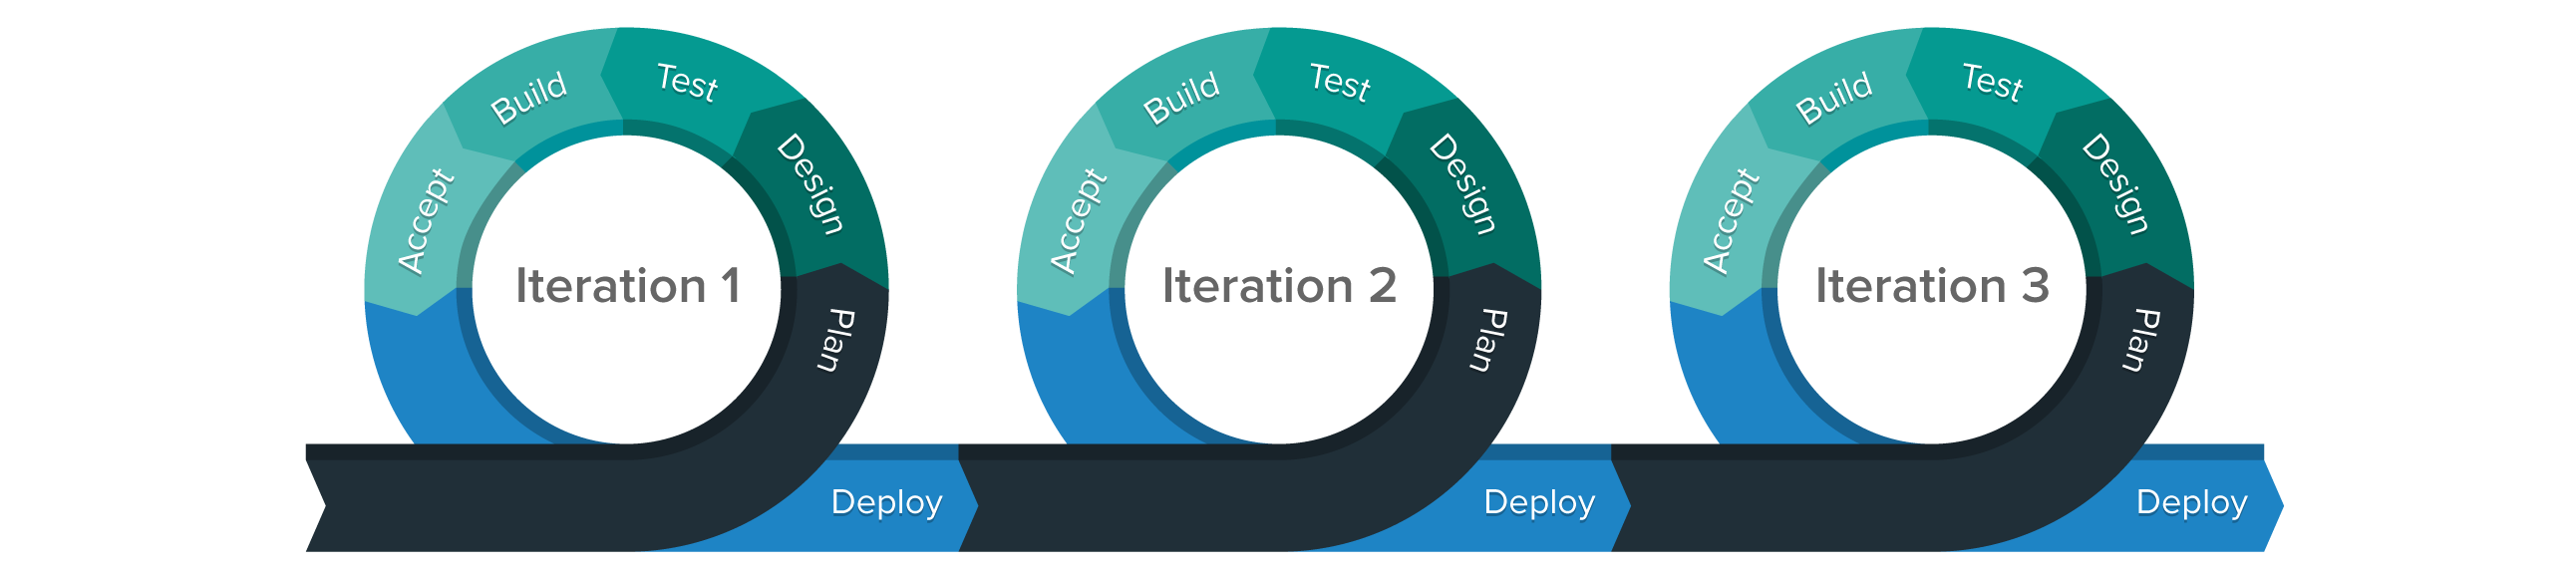
\includegraphics[width=\textwidth]{images/agile-methodolody.png}
    \caption{Iterations using Agile methodology}
    \label{fig:agile-methodology}
\end{figure}

A good summary of the Agile methodology is the agile manifesto\cite{agilemanifesto}, that states the main principles of this methodology.

\begin{bclogo}[logo=\bctrombone]{Agile Manifesto \cite{agilemanifesto}}
\emph{Individuals and interactions} over processes and tools.\\
\emph{Working software} over comprehensive documentation.\\
\emph{Customer collaboration} over contract negotiation.\\
\emph{Responding to change} over following a plan. \\
That is, while there is value in the items on
the right, we value the items on the left more.
\end{bclogo}

The main advantages of this methodology are to have flexibility and regular feedback on the product delivered.

\paragraph{Python}
Python is a programming language used in many fields. Its main advantage is great readability.

\todo[inline]{Talk more about python? Creator, specificity's, interpreted language, speed, community, TIOBE Index...? \url{ https://www.tiobe.com/tiobe-index/} Mainly explain why you chose it and what its main features/specificities you will rely upon}

\paragraph{Software framework}

A framework is a set of tools that provides features that can be reused in multiple applications. A framework is different from a library in the sense that when using a library, we call the methods of the library while when using a framework, our code is called by the framework. The difference is shown on figure \ref{fig:framework-vs-library}. Frameworks help to build reusable and maintainable applications 
\todo[inline]{give some examples of frameworks + why you talk about it, integrate Django with it?}

\begin{figure}
    \centering
    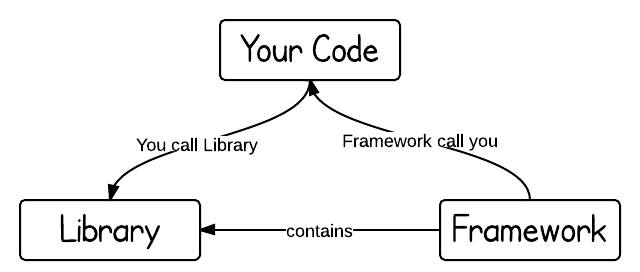
\includegraphics[width=0.5\textwidth]{images/framework-vs-library.png}
    \caption{Framework versus library}
    \label{fig:framework-vs-library}
\end{figure}
\paragraph{Django}
Django is a web framework to develop web applications in Python. 
\todo[inline]{Develop, why django, what others, what features of Djangos do you rely upon, what plugins, and so on}

\paragraph{Continuous Integration}
Continuous integration (often referred as CI) is a software engineering practice to help development teams working on a set repository. 
When using CI, we automate a set of checks at each push request on a repository and developers should merge to this repository regularly. With continuous integration, we will detect bugs faster and more easily. We can also add tests to our continuous integration tool, these tests will then be run at each push request and we will receive a notification if they fail. Thanks to that, we can see exactly which commit implied a failure in the tests. If we do small regular commits, it will be really easy to find where the failure comes from.

\todo[inline]{Why you explain this, what CI you use, what CI features and tools you use; why you use these}